
\begin{frame}{Intuitivement...}
	Le graphe est assimilé à un réseau de tuyaux de capacité donnée.\vfill
\end{frame}

\begin{frame}{Intuitivement...}
	Le graphe est assimilé à un réseau de tuyaux de capacité donnée.\vfill
	Chaque noeud possède un réservoir de capacité infinie.\vfill
\end{frame}

\begin{frame}{Intuitivement...}
	Le graphe est assimilé à un réseau de tuyaux de capacité donnée.\vfill
	Chaque noeud possède un réservoir de capacité infinie.\vfill
	Seule la source possède un réservoir plein. \vfill
\end{frame}

\begin{frame}{Intuitivement...}
	Le graphe est assimilé à un réseau de tuyaux de capacité donnée.\vfill
	Chaque noeud possède un réservoir de capacité infinie.\vfill
	Seule la source possède un réservoir plein. \vfill
	À chaque noeud est associée une hauteur.\vfill
\end{frame}

\begin{frame}{Intuitivement...}
	Le graphe est assimilé à un réseau de tuyaux de capacité donnée.\vfill
	Chaque noeud possède un réservoir de capacité infinie.\vfill
	Seule la source possède un réservoir plein. \vfill
	À chaque noeud est associée une hauteur.\vfill
	Deux actions possibles : \begin{enumerate}
		\item vidange du réservoir
	\end{enumerate} \vfill
\end{frame}

\begin{frame}{Intuitivement...}
	Le graphe est assimilé à un réseau de tuyaux de capacité donnée.\vfill
	Chaque noeud possède un réservoir de capacité infinie.\vfill
	Seule la source possède un réservoir plein. \vfill
	À chaque noeud est associée une hauteur.\vfill
	Deux actions possibles : \begin{enumerate}
		\item vidange du réservoir
		\item augmentation de la hauteur du réservoir
	\end{enumerate} \vfill
\end{frame}

\begin{frame}{Intuitivement...}
	Le graphe est assimilé à un réseau de tuyaux de capacité donnée.\vfill
	Chaque noeud possède un réservoir de capacité infinie.\vfill
	Seule la source possède un réservoir plein. \vfill
	À chaque noeud est associée une hauteur.\vfill
	Deux actions possibles : \begin{enumerate}
		\item vidange du réservoir
		\item augmentation de la hauteur du réservoir
	\end{enumerate} \vfill
	On commence par vidanger la source, puis on cherche à vidanger les noeuds dont le réservoir n'est
	pas vide. \vfill
\end{frame}

\begin{frame}{Intuitivement...}
	Le graphe est assimilé à un réseau de tuyaux de capacité donnée.\vfill
	Chaque noeud possède un réservoir de capacité infinie.\vfill
	Seule la source possède un réservoir plein. \vfill
	À chaque noeud est associée une hauteur.\vfill
	Deux actions possibles : \begin{enumerate}
		\item vidange du réservoir
		\item augmentation de la hauteur du réservoir
	\end{enumerate} \vfill
	On commence par vidanger la source, puis on cherche à vidanger les noeuds dont le réservoir n'est
	pas vide. \vfill
	Si on ne peut vidanger aucun réservoir et qu'il reste des réservoirs non vides, on augmente la
	hauteur de ces derniers. \vfill
\end{frame}


\subsection{Définitions}
\begin{frame}{La notion de préflot}
	Un préflot est une fonction obtenue à partir d'un flot par relaxation de la loi de Kirchoff : la
	quantité de préflot sortant d'un noeud doit être inférieure ou égale à la quantité de préflot
	entrant dans celui-ci.\vfill
\end{frame}

\begin{frame}{La notion de préflot}
	Un préflot est une fonction obtenue à partir d'un flot par relaxation de la loi de Kirchoff : la
	quantité de préflot sortant d'un noeud doit être inférieure ou égale à la quantité de préflot
	entrant dans celui-ci.\vfill
	\begin{minipage}[c]{0.45\linewidth}
		\begin{figure}
			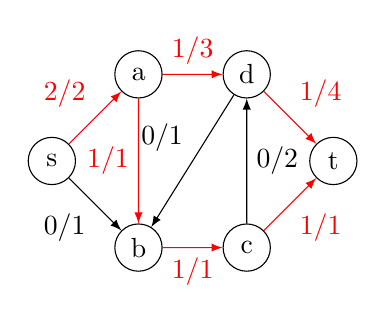
\begin{tikzpicture}[scale=0.55]
				\tikzset{noeud/.style={circle, draw=black, inner sep=0.1cm, minimum width=0.6cm}, fleche/.style={>=latex, ->}};
				\node[noeud] (s) at (0,0) {s};
				\node[noeud] (a) at (2, 2) {a};
				\node[noeud] (b) at (2, -2) {b};
				\node[noeud] (c) at (4.5, -2) {c};
				\node[noeud] (d) at (4.5, 2) {d};
				\node[noeud] (t) at (6.5,0) {t};

				\draw[fleche, red] (s) -- node[above left, red] {$2/2$}(a);
				\draw[fleche] (s) -- node[below left] {$0/1$}(b);
				\draw[fleche, red] (a) -- node[left,red] {$1/1$}(b);
				\draw[fleche, red] (a) -- node[above, red] {$1/3$}(d);
				\draw[fleche] (d) -- node[above left] {$0/1$}(b);
				\draw[fleche, red] (b) -- node[below, red] {$1/1$}(c);
				\draw[fleche, red] (d) -- node[above right, red] {$1/4$}(t);
				\draw[fleche, red] (c) -- node[below right, red] {$1/1$}(t);
				\draw[fleche] (c) -- node[right] {$0/2$}(d);
			\end{tikzpicture}
			\caption{Un exemple de flot}
		\end{figure}
	\end{minipage} \hfill
	\begin{minipage}[c]{0.45\linewidth}
	\end{minipage}
\end{frame}

\begin{frame}{La notion de préflot}
	Un préflot est une fonction obtenue à partir d'un flot par relaxation de la loi de Kirchoff : la
	quantité de préflot sortant d'un noeud doit être inférieure ou égale à la quantité de préflot
	entrant dans celui-ci.\vfill
	\begin{minipage}[c]{0.45\linewidth}
		\begin{figure}
			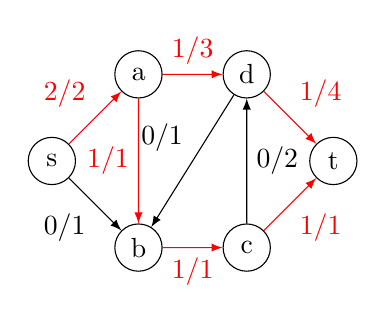
\begin{tikzpicture}[scale=0.55]
				\tikzset{noeud/.style={circle, draw=black, inner sep=0.1cm, minimum width=0.6cm}, fleche/.style={>=latex, ->}};
				\node[noeud] (s) at (0,0) {s};
				\node[noeud] (a) at (2, 2) {a};
				\node[noeud] (b) at (2, -2) {b};
				\node[noeud] (c) at (4.5, -2) {c};
				\node[noeud] (d) at (4.5, 2) {d};
				\node[noeud] (t) at (6.5,0) {t};

				\draw[fleche, red] (s) -- node[above left, red] {$2/2$}(a);
				\draw[fleche] (s) -- node[below left] {$0/1$}(b);
				\draw[fleche, red] (a) -- node[left,red] {$1/1$}(b);
				\draw[fleche, red] (a) -- node[above, red] {$1/3$}(d);
				\draw[fleche] (d) -- node[above left] {$0/1$}(b);
				\draw[fleche, red] (b) -- node[below, red] {$1/1$}(c);
				\draw[fleche, red] (d) -- node[above right, red] {$1/4$}(t);
				\draw[fleche, red] (c) -- node[below right, red] {$1/1$}(t);
				\draw[fleche] (c) -- node[right] {$0/2$}(d);
			\end{tikzpicture}
			\caption{Un exemple de flot}
		\end{figure}
	\end{minipage} \hfill
	\begin{minipage}[c]{0.45\linewidth}
		\begin{figure}
			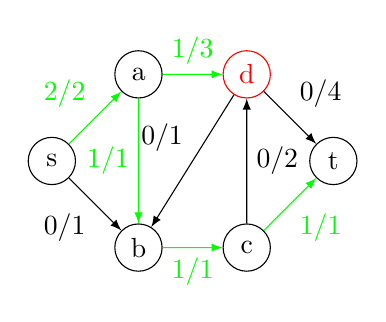
\begin{tikzpicture}[scale=0.55]
				\tikzset{noeud/.style={circle, draw=black, inner sep=0.1cm, minimum width=0.6cm}, fleche/.style={>=latex, ->}};
				\node[noeud] (s) at (0,0) {s};
				\node[noeud] (a) at (2, 2) {a};
				\node[noeud] (b) at (2, -2) {b};
				\node[noeud] (c) at (4.5, -2) {c};
				\node[noeud, draw=red, red] (d) at (4.5, 2) {d};
				\node[noeud] (t) at (6.5,0) {t};

				\draw[fleche, green] (s) -- node[above left, green] {$2/2$}(a);
				\draw[fleche] (s) -- node[below left] {$0/1$}(b);
				\draw[fleche, green] (a) -- node[left,green] {$1/1$}(b);
				\draw[fleche, green] (a) -- node[above, green] {$1/3$}(d);
				\draw[fleche] (d) -- node[above left] {$0/1$}(b);
				\draw[fleche, green] (b) -- node[below, green] {$1/1$}(c);
				\draw[fleche] (d) -- node[above right] {$0/4$}(t);
				\draw[fleche, green] (c) -- node[below right, green] {$1/1$}(t);
				\draw[fleche] (c) -- node[right] {$0/2$}(d);
			\end{tikzpicture}
			\caption{Un exemple de préflot}
		\end{figure}
	\end{minipage}
\end{frame}

\begin{frame}{La notion de préflot}
	Un préflot est une fonction obtenue à partir d'un flot par relaxation de la loi de Kirchoff : la
	quantité de préflot sortant d'un noeud doit être inférieure ou égale à la quantité de préflot
	entrant dans celui-ci.\vfill
	\begin{minipage}[c]{0.45\linewidth}
		\begin{figure}
			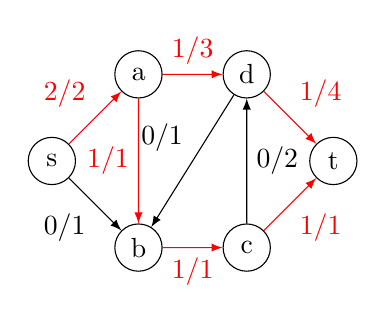
\begin{tikzpicture}[scale=0.55]
				\tikzset{noeud/.style={circle, draw=black, inner sep=0.1cm, minimum width=0.6cm}, fleche/.style={>=latex, ->}};
				\node[noeud] (s) at (0,0) {s};
				\node[noeud] (a) at (2, 2) {a};
				\node[noeud] (b) at (2, -2) {b};
				\node[noeud] (c) at (4.5, -2) {c};
				\node[noeud] (d) at (4.5, 2) {d};
				\node[noeud] (t) at (6.5,0) {t};

				\draw[fleche, red] (s) -- node[above left, red] {$2/2$}(a);
				\draw[fleche] (s) -- node[below left] {$0/1$}(b);
				\draw[fleche, red] (a) -- node[left,red] {$1/1$}(b);
				\draw[fleche, red] (a) -- node[above, red] {$1/3$}(d);
				\draw[fleche] (d) -- node[above left] {$0/1$}(b);
				\draw[fleche, red] (b) -- node[below, red] {$1/1$}(c);
				\draw[fleche, red] (d) -- node[above right, red] {$1/4$}(t);
				\draw[fleche, red] (c) -- node[below right, red] {$1/1$}(t);
				\draw[fleche] (c) -- node[right] {$0/2$}(d);
			\end{tikzpicture}
			\caption{Un exemple de flot}
		\end{figure}
	\end{minipage} \hfill
	\begin{minipage}[c]{0.45\linewidth}
		\begin{figure}
			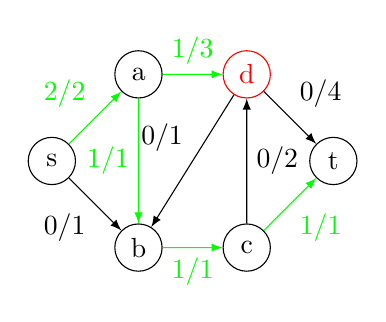
\begin{tikzpicture}[scale=0.55]
				\tikzset{noeud/.style={circle, draw=black, inner sep=0.1cm, minimum width=0.6cm}, fleche/.style={>=latex, ->}};
				\node[noeud] (s) at (0,0) {s};
				\node[noeud] (a) at (2, 2) {a};
				\node[noeud] (b) at (2, -2) {b};
				\node[noeud] (c) at (4.5, -2) {c};
				\node[noeud, draw=red, red] (d) at (4.5, 2) {d};
				\node[noeud] (t) at (6.5,0) {t};

				\draw[fleche, green] (s) -- node[above left, green] {$2/2$}(a);
				\draw[fleche] (s) -- node[below left] {$0/1$}(b);
				\draw[fleche, green] (a) -- node[left,green] {$1/1$}(b);
				\draw[fleche, green] (a) -- node[above, green] {$1/3$}(d);
				\draw[fleche] (d) -- node[above left] {$0/1$}(b);
				\draw[fleche, green] (b) -- node[below, green] {$1/1$}(c);
				\draw[fleche] (d) -- node[above right] {$0/4$}(t);
				\draw[fleche, green] (c) -- node[below right, green] {$1/1$}(t);
				\draw[fleche] (c) -- node[right] {$0/2$}(d);
			\end{tikzpicture}
			\caption{Un exemple de préflot}
		\end{figure}
	\end{minipage}
	\begin{alertblock}{Définition}
	$e(d) = f_{in} - f_{out} = 1$. d est appelé noeud actif et $e(d)$, l'excédent de d.
	\end{alertblock} \vfill
\end{frame}

\begin{frame}{La fonction de distance}
	Une fonction de distance est une fonction représentant le plus court chemin en nombre d'arcs d'un
	noeud au puits, vérifiant les propriétés suivantes :\vfill
\end{frame}

\begin{frame}{La fonction de distance}
	Une fonction de distance est une fonction représentant le plus court chemin en nombre d'arcs d'un
	noeud au puits, vérifiant les propriétés suivantes : \vfill
	\begin{exampleblock}{Distance de la source}
		la distance de la source est égale au nombre de sommets du graphe
	\end{exampleblock} \vfill
\end{frame}

\begin{frame}{La fonction de distance}
	Une fonction de distance est une fonction représentant le plus court chemin en nombre d'arcs d'un
	noeud au puits, vérifiant les propriétés suivantes : \vfill
	\begin{block}{Propriétés}
		$$ d(s) = |S| $$
	\end{block} \vfill
	\begin{exampleblock}{Distance du puits}
		la distance du puits est égale à zéro
	\end{exampleblock} \vfill
\end{frame}

\begin{frame}{La fonction de distance}
	Une fonction de distance est une fonction représentant la distance d'un noeud au puits, vérifiant
	les propriétés suivantes : \vfill
	\begin{block}{Propriétés}
		$$ d(s) = |S| $$
		$$ d(t) = 0 $$
	\end{block} \vfill
	\begin{exampleblock}{Distances des sommets}
		si $(i,j)$ appartient au réseau résiduel, la distance du sommet $i$ est égale à la distance du sommet $i$ plus un
	\end{exampleblock}
\end{frame}

\begin{frame}{La fonction de distance}
	Une fonction de distance est une fonction représentant la distance d'un noeud au puits, vérifiant
	les propriétés suivantes : \vfill
	\begin{block}{Propriétés}
		$$ d(s) = |S| $$
		$$ d(t) = 0 $$
		$$ \forall (i,j) \in A_f,\quad d(i) = d(j) + 1 $$
	\end{block}
\end{frame}

\begin{frame}{Conséquences sur le réseau résiduel}
	Le réseau résiduel associé au flot suivant : \vfill
	\begin{minipage}[c]{0.45\linewidth}
		\begin{figure}
			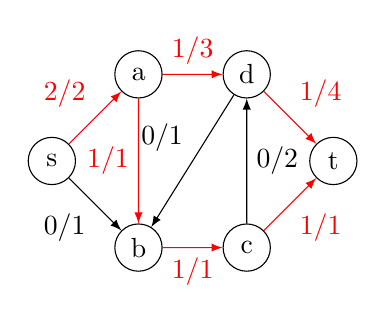
\begin{tikzpicture}[scale=0.55]
				\tikzset{noeud/.style={circle, draw=black, inner sep=0.1cm, minimum width=0.6cm}, fleche/.style={>=latex, ->}};
				\node[noeud] (s) at (0,0) {s};
				\node[noeud] (a) at (2, 2) {a};
				\node[noeud] (b) at (2, -2) {b};
				\node[noeud] (c) at (4.5, -2) {c};
				\node[noeud] (d) at (4.5, 2) {d};
				\node[noeud] (t) at (6.5,0) {t};

				\draw[fleche, red] (s) -- node[above left, red] {$2/2$}(a);
				\draw[fleche] (s) -- node[below left] {$0/1$}(b);
				\draw[fleche, red] (a) -- node[left,red] {$1/1$}(b);
				\draw[fleche, red] (a) -- node[above, red] {$1/3$}(d);
				\draw[fleche] (d) -- node[above left] {$0/1$}(b);
				\draw[fleche, red] (b) -- node[below, red] {$1/1$}(c);
				\draw[fleche, red] (d) -- node[above right, red] {$1/4$}(t);
				\draw[fleche, red] (c) -- node[below right, red] {$1/1$}(t);
				\draw[fleche] (c) -- node[right] {$0/2$}(d);
			\end{tikzpicture}
			\caption{Un exemple de flot}
		\end{figure}
	\end{minipage} \hfill
	\begin{minipage}[c]{0.45\linewidth}
	\end{minipage}
\end{frame}

\begin{frame}{Conséquences sur le réseau résiduel}
	devient : \vfill
	\begin{minipage}[c]{0.45\linewidth}
		\begin{figure}
			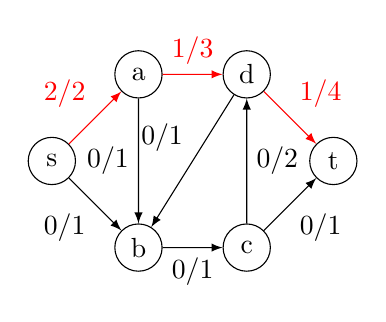
\begin{tikzpicture}[scale=0.55]
				\tikzset{noeud/.style={circle, draw=black, inner sep=0.1cm, minimum width=0.6cm}, fleche/.style={>=latex, ->}};
				\node[noeud] (s) at (0,0) {s};
				\node[noeud] (a) at (2, 2) {a};
				\node[noeud] (b) at (2, -2) {b};
				\node[noeud] (c) at (4.5, -2) {c};
				\node[noeud] (d) at (4.5, 2) {d};
				\node[noeud] (t) at (6.5,0) {t};

				\draw[fleche, red] (s) -- node[above left, red] {$2/2$}(a);
				\draw[fleche] (s) -- node[below left] {$0/1$}(b);
				\draw[fleche] (a) -- node[left] {$0/1$}(b);
				\draw[fleche, red] (a) -- node[above, red] {$1/3$}(d);
				\draw[fleche] (d) -- node[above left] {$0/1$}(b);
				\draw[fleche] (b) -- node[below] {$0/1$}(c);
				\draw[fleche, red] (d) -- node[above right, red] {$1/4$}(t);
				\draw[fleche] (c) -- node[below right] {$0/1$}(t);
				\draw[fleche] (c) -- node[right] {$0/2$}(d);
			\end{tikzpicture}
			\caption{Un exemple de flot}
		\end{figure}
	\end{minipage} \hfill
	\begin{minipage}[c]{0.45\linewidth}
		\begin{figure}
			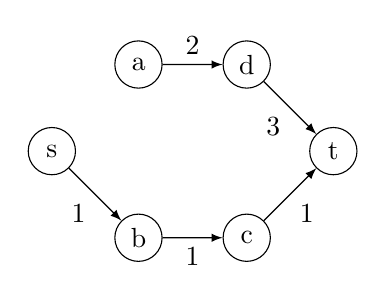
\begin{tikzpicture}[scale=0.55]
				\tikzset{noeud/.style={circle, draw=black, inner sep=0.1cm, minimum width=0.6cm}, fleche/.style={>=latex, ->}};
				\node[noeud] (s) at (0,0) {s};
				\node[noeud] (a) at (2, 2) {a};
				\node[noeud] (b) at (2, -2) {b};
				\node[noeud] (c) at (4.5, -2) {c};
				\node[noeud] (d) at (4.5, 2) {d};
				\node[noeud] (t) at (6.5,0) {t};

				\draw[fleche] (s) -- node[below left] {$1$}(b);
				\draw[fleche] (a) to node[above] {$2$}(d);
				\draw[fleche] (d) to node[below left] {$3$}(t);
				\draw[fleche] (c) -- node[below right] {$1$}(t);
				\draw[fleche] (b) -- node[below] {$1$}(c);
			\end{tikzpicture}
			\caption{Le réseau résiduel associé}
		\end{figure}
	\end{minipage}
\end{frame}

\begin{frame}{Conséquences sur le réseau résiduel}
	devient : \vfill
	\begin{minipage}[c]{0.45\linewidth}
		\begin{figure}
			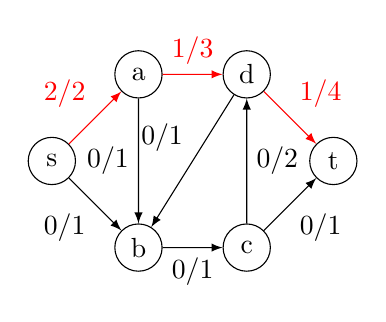
\begin{tikzpicture}[scale=0.55]
				\tikzset{noeud/.style={circle, draw=black, inner sep=0.1cm, minimum width=0.6cm}, fleche/.style={>=latex, ->}};
				\node[noeud] (s) at (0,0) {s};
				\node[noeud] (a) at (2, 2) {a};
				\node[noeud] (b) at (2, -2) {b};
				\node[noeud] (c) at (4.5, -2) {c};
				\node[noeud] (d) at (4.5, 2) {d};
				\node[noeud] (t) at (6.5,0) {t};

				\draw[fleche, red] (s) -- node[above left, red] {$2/2$}(a);
				\draw[fleche] (s) -- node[below left] {$0/1$}(b);
				\draw[fleche] (a) -- node[left] {$0/1$}(b);
				\draw[fleche, red] (a) -- node[above, red] {$1/3$}(d);
				\draw[fleche] (d) -- node[above left] {$0/1$}(b);
				\draw[fleche] (b) -- node[below] {$0/1$}(c);
				\draw[fleche, red] (d) -- node[above right, red] {$1/4$}(t);
				\draw[fleche] (c) -- node[below right] {$0/1$}(t);
				\draw[fleche] (c) -- node[right] {$0/2$}(d);
			\end{tikzpicture}
			\caption{Un exemple de flot}
		\end{figure}
	\end{minipage} \hfill
	\begin{minipage}[c]{0.45\linewidth}
		\begin{figure}
			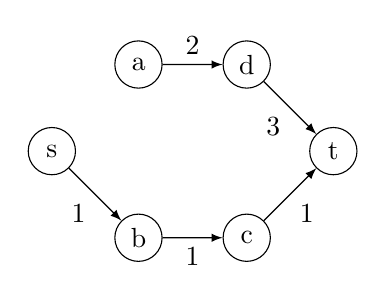
\begin{tikzpicture}[scale=0.55]
				\tikzset{noeud/.style={circle, draw=black, inner sep=0.1cm, minimum width=0.6cm}, fleche/.style={>=latex, ->}};
				\node[noeud] (s) at (0,0) {s};
				\node[noeud] (a) at (2, 2) {a};
				\node[noeud] (b) at (2, -2) {b};
				\node[noeud] (c) at (4.5, -2) {c};
				\node[noeud] (d) at (4.5, 2) {d};
				\node[noeud] (t) at (6.5,0) {t};

				\draw[fleche] (s) -- node[below left] {$1$}(b);
				\draw[fleche] (a) to node[above] {$2$}(d);
				\draw[fleche] (d) to node[below left] {$3$}(t);
				\draw[fleche] (c) -- node[below right] {$1$}(t);
				\draw[fleche] (b) -- node[below] {$1$}(c);
			\end{tikzpicture}
			\caption{Le réseau résiduel associé}
		\end{figure}
	\end{minipage}
	\begin{exampleblock}{Note}
		Le réseau résiduel sert à déterminer les actions à effectuer.
	\end{exampleblock}
\end{frame}

\subsection{Principe}
\begin{frame}{Poussage}
	\textbf{Poussage :} L'action de faire transiter le préflot d'un noeud $i$ à un noeud $j$ est appelée
	opération de poussage.\\
\end{frame}

\begin{frame}{Poussage}
	\textbf{Poussage :} L'action de faire transiter le préflot d'un noeud $i$ à un noeud $j$ est appelée
	opération de poussage.\\
	\begin{alertblock}{Condition}
		On ne peut pas appliquer un poussage sur l'arrête $(i,j)$ que si le sommet $i$ est
		actif, $C_f$ $(i,j)>0$ et $d(i) = d(j)$ + 1.\\
	\end{alertblock}
\end{frame}

\begin{frame}{Insuffisance des poussages}
	Soit le graphe :\vfill

	\begin{figure}
	\begin{center}
		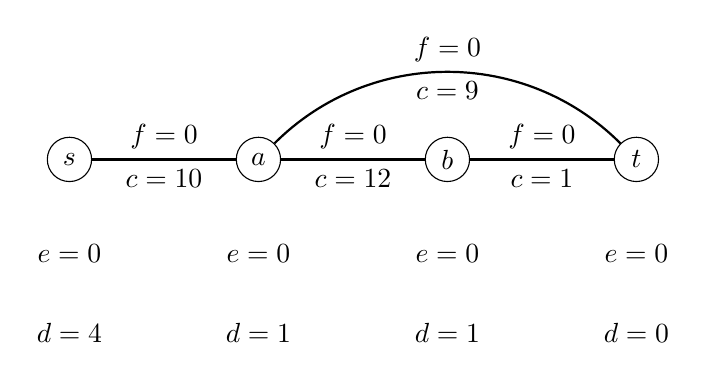
\begin{tikzpicture}[scale=0.6, node distance = 1cm]
			\tikzset{noeud/.style={circle, draw=black, text centered,minimum size=16pt, inner sep=0pt},
			fleche/.style={thick,>=latex}};

			\foreach \name/\x/\exc\dist in {s/0/0/4, a/4/0/1, b/8/0/1, t/12/0/0}{
				\node[noeud] (\name) at (\x, 1) {$\name$};
				\node (e-\name) at (\x, -1) {$e=\exc$};
				\node (d-\name) [below of=e-\name] {$d=\dist$};
			}

			\draw[fleche] (s) -- node[above] {$f=  0$} node[below] {$c=10$} (a);
			\draw[fleche] (a) -- node[above] {$f=  0$} node[below] {$c=12$} (b);
			\draw[fleche] (b) -- node[above] {$f=  0$} node[below] {$c= 1$} (t);
			\draw[fleche] (a) to[out=45, in=135]	node[above] {$f=0$} node[below] {$c= 9$} (t);

		\end{tikzpicture}
	\end{center}
\end{figure} \vfill
\end{frame}

\begin{frame}{Insuffisance des poussages}
	Soit le graphe :\vfill

	\begin{figure}
	\begin{center}
		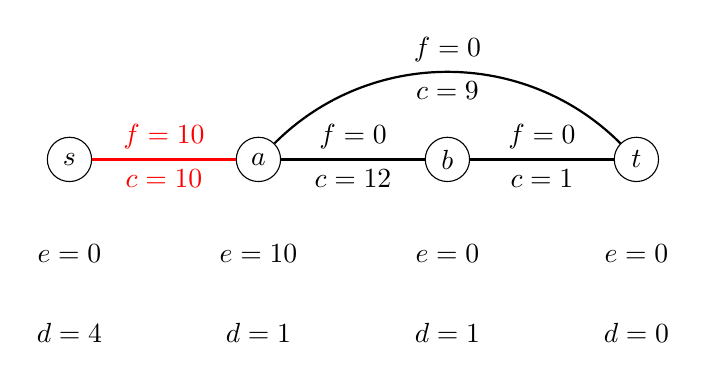
\begin{tikzpicture}[scale=0.6, node distance = 1cm]
			\tikzset{noeud/.style={circle, draw=black, text centered,minimum size=16pt, inner sep=0pt},
			fleche/.style={thick, >=latex}};

			\foreach \name/\x/\exc\dist in {s/0/0/4, a/4/10/1, b/8/0/1, t/12/0/0}{
				\node[noeud] (\name) at (\x, 1) {$\name$};
				\node (e-\name) at (\x, -1) {$e=\exc$};
				\node (d-\name) [below of=e-\name] {$d=\dist$};
			}

			\draw[fleche, red] (s) -- node[above, red] {$f=  10$} node[below] {$c=10$} (a);
			\draw[fleche] (a) -- node[above] {$f=  0$} node[below] {$c=12$} (b);
			\draw[fleche] (b) -- node[above] {$f=  0$} node[below] {$c= 1$} (t);
			\draw[fleche] (a) to[out=45, in=135]	node[above] {$f=0$} node[below] {$c= 9$} (t);

		\end{tikzpicture}
	\end{center}
\end{figure} \vfill
\end{frame}

\begin{frame}{Insuffisance des poussages}
	Soit le graphe :\vfill

	\begin{figure}
	\begin{center}
		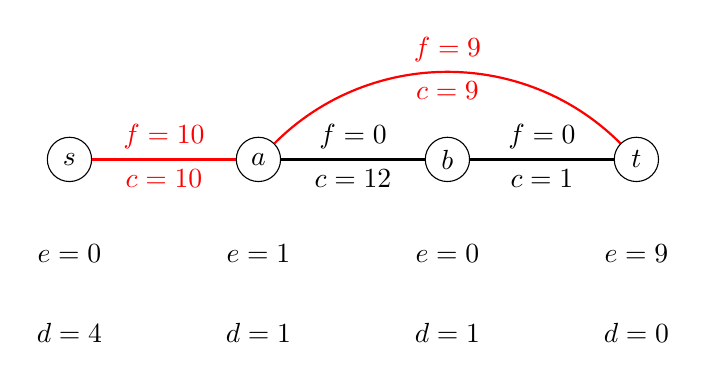
\begin{tikzpicture}[scale=0.6, node distance = 1cm]
			\tikzset{noeud/.style={circle, draw=black, text centered,minimum size=16pt, inner sep=0pt},
			fleche/.style={thick, >=latex}};

			\foreach \name/\x/\exc\dist in {s/0/0/4, a/4/1/1, b/8/0/1, t/12/9/0}{
				\node[noeud] (\name) at (\x, 1) {$\name$};
				\node (e-\name) at (\x, -1) {$e=\exc$};
				\node (d-\name) [below of=e-\name] {$d=\dist$};
			}

			\draw[fleche, red] (s) -- node[above, red] {$f=  10$} node[below] {$c=10$} (a);
			\draw[fleche] (a) -- node[above] {$f=  0$} node[below] {$c=12$} (b);
			\draw[fleche] (b) -- node[above] {$f=  0$} node[below] {$c= 1$} (t);
			\draw[fleche, red] (a) to[out=45, in=135]	node[above, red] {$f=9$} node[below] {$c= 9$} (t);

		\end{tikzpicture}
	\end{center}
\end{figure} \vfill
\end{frame}

\begin{frame}{Insuffisance des poussages}
	Soit le graphe :\vfill

	\begin{figure}
	\begin{center}
		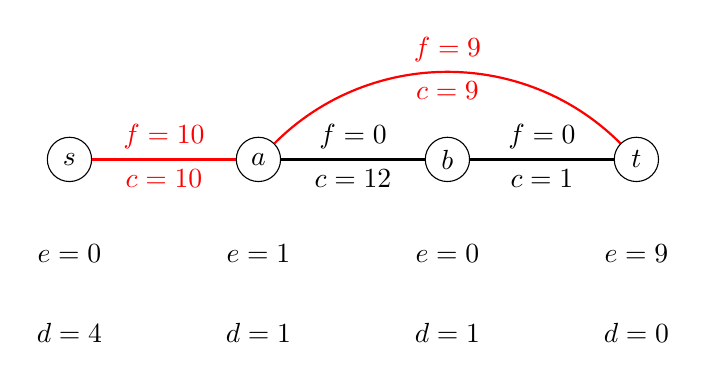
\begin{tikzpicture}[scale=0.6, node distance = 1cm]
			\tikzset{noeud/.style={circle, draw=black, text centered,minimum size=16pt, inner sep=0pt},
			fleche/.style={thick, >=latex}};

			\foreach \name/\x/\exc\dist in {s/0/0/4, a/4/1/1, b/8/0/1, t/12/9/0}{
				\node[noeud] (\name) at (\x, 1) {$\name$};
				\node (e-\name) at (\x, -1) {$e=\exc$};
				\node (d-\name) [below of=e-\name] {$d=\dist$};
			}

			\draw[fleche, red] (s) -- node[above, red] {$f=  10$} node[below] {$c=10$} (a);
			\draw[fleche] (a) -- node[above] {$f=  0$} node[below] {$c=12$} (b);
			\draw[fleche] (b) -- node[above] {$f=  0$} node[below] {$c= 1$} (t);
			\draw[fleche, red] (a) to[out=45, in=135]	node[above, red] {$f=9$} node[below] {$c= 9$} (t);

		\end{tikzpicture}
	\end{center}
\end{figure} \vfill
\begin{block}{Et maintenant ...}
	Que faire ?
\end{block}
\end{frame}

\begin{frame}{Réétiquetage}
	\textbf{Réétiquetage :} Le ré-étiquetage consiste à réévaluer la distance du noeud actif au
	noeud puits afin qu'il soit possible, après cette opération, d'effectuer une opération de
	poussage depuis ce noeud.
\end{frame}

\begin{frame}{Réétiquetage}
	\textbf{Réétiquetage :} Le ré-étiquetage consiste à réévaluer la distance du noeud actif au
	noeud puits afin qu'il soit possible, après cette opération, d'effectuer une opération de
	poussage depuis ce noeud.
	\begin{alertblock}{Condition}
		On ne peut pas réétiqueter que si $i$ est actif et, pour tout $j \in S$ tel
		que $(i,j) \in A_f$. On a $d (i)\leq d (j)$. 
	\end{alertblock}
\end{frame}

\begin{frame}{Approche formelle}
	L'algorithme examine les noeuds actifs.\vfill
\end{frame}

\begin{frame}{Approche formelle}
	L'algorithme examine les noeuds actifs.\vfill
	Il cherche à réduire l'excédent de flot en l'envoyant vers un noeud voisin dans le graphe
	résiduel (Poussage).\vfill
\end{frame}

\begin{frame}{Approche formelle}
	L'algorithme examine les noeuds actifs.\vfill
	Il cherche à réduire l'excédent de flot en l'envoyant vers un noeud voisin dans le graphe
	résiduel (Poussage).\vfill
	S'il n'existe aucun voisin, on augmente la distance du noeud au puits (Ré-étiquetage).\vfill
\end{frame}

\begin{frame}{Approche formelle}
	L'algorithme examine les noeuds actifs.\vfill
	Il cherche à réduire l'excédent de flot en l'envoyant vers un noeud voisin dans le graphe
	résiduel (Poussage).\vfill
	S'il n'existe aucun voisin, on augmente la distance du noeud au puits (Ré-étiquetage).\vfill
	Lorsque plus aucun noeud est actif, le préflot restant est un flot maximum.\vfill
\end{frame}


